\newpage
\section{Washing Machine}

\subsection{Mathematical Representation}

\noindent The EFSM of the washing machine is the tuple $S = (Q, \Sigma_1, \Sigma_2, q_0, V, \Lambda)$, where\\

\noindent $Q = \{Off, On, Operating\}$\\
\noindent $\Sigma_1 = \{turn on, after(10sec), shut down\}$\\
\noindent $\Sigma_2 = \{operating~lights~blink, beep, long~beep, operating~lights~off\}$\\
\noindent $q_0: Off$\\
\noindent $V: \emptyset$\\
\noindent $\Lambda$: Transition specifications\\
\indent 1. $\rightarrow Off$\\
\indent 2. $Off \xrightarrow {\text { turnOn}} On$\\
\indent 3. $On \xrightarrow {\text { after(10sec) / operating lights blink; long beep}} Operating$\\
\indent 4. $Operating \xrightarrow {\text { shutDown / beep; operating lights off}} Off$\\

\noindent The UML state diagram is shown in Figure~\ref{fig:washingMachine}.


\subsection{State transition diagram}

\begin{figure}[h!]
	\centering
		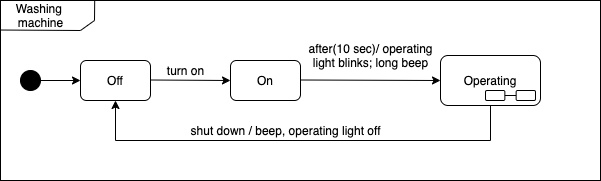
\includegraphics[width=0.8\textwidth]{WashingMachine}
		  \caption{Washing Machine State Diagram}
  \label{fig:washingMachine}
\end{figure}
